\documentclass[a4paper,12pt]{article} 
\usepackage[utf8]{inputenc}
\usepackage[T1]{fontenc}
\usepackage{amsmath,amssymb,amsthm}
\usepackage{xcolor}
\usepackage{tikz} 
\usetikzlibrary {arrows.meta}
\usetikzlibrary{shapes.geometric}
\usetikzlibrary{bending}

\begin{document}

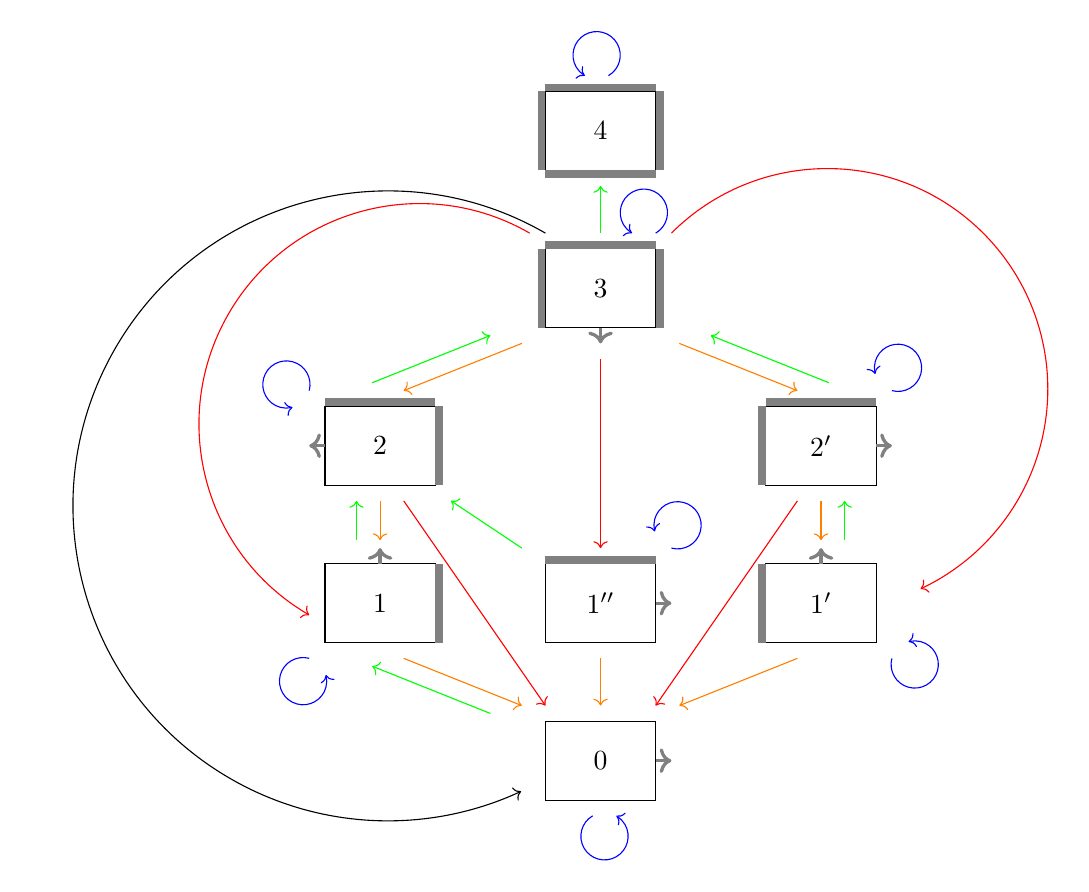
\begin{tikzpicture}
    \draw (0, 0) rectangle (1.4, 1) node[midway] {$0$};
    \draw[->, very thick, gray] (1.4, .5) -> ++(.2,0);
    \draw (0, 2) rectangle (1.4, 3) node[midway] {$1''$};
    \draw[->, very thick, gray] (1.4, 2.5) -> ++(.2,0);
    \fill[gray] (0, 3) rectangle (1.4, 3.1);
    \draw (0, 6) rectangle (1.4, 7) node[midway] {$3$};
    \draw[->, very thick, gray] (.7, 6) -> ++(0,-.2);
    \fill[gray] (1.4, 6) rectangle (1.5, 7);
    \fill[gray] (0, 7) rectangle (1.4, 7.1);
    \fill[gray] (-.1, 6) rectangle (0, 7);
    \draw (0, 8) rectangle (1.4, 9) node[midway] {$4$};
    \fill[gray] (1.4, 8) rectangle (1.5, 9);
    \fill[gray] (0, 9) rectangle (1.4, 9.1);
    \fill[gray] (-.1, 8) rectangle (0, 9);
    \fill[gray] (0, 7.9) rectangle (1.4, 8);
    \draw (-2.8, 2) rectangle (-1.4, 3) node[midway] {$1$};
    \draw[->, very thick, gray] (-2.1, 3) -> ++(0,.2);
    \fill[gray] (-1.4, 2) rectangle (-1.3, 3);
    \draw (-2.8, 4) rectangle (-1.4, 5) node[midway] {$2$};
    \draw[->, very thick, gray] (-2.8, 4.5) -> ++(-.2, 0);
    \fill[gray] (-1.4, 4) rectangle (-1.3, 5);
    \fill[gray] (-2.8, 5) rectangle (-1.4, 5.1);
    \draw (2.8, 2) rectangle (4.2, 3) node[midway] {$1'$};
    \draw[->, very thick, gray] (3.5, 3) -> ++(0,.2);
    \fill[gray] (2.8, 2) rectangle (2.7, 3);
    \draw (2.8, 4) rectangle (4.2, 5) node[midway] {$2'$};
    \draw[->, very thick, gray] (4.2, 4.5) -> ++(.2, 0);
    \fill[gray] (2.8, 4) rectangle (2.7, 5);
    \fill[gray] (2.8, 5) rectangle (4.2, 5.1);
    \path[->,orange] (.7, 1.8) edge (.7, 1.2);    % 1' -> 0
    \path[<-,green] (.7, 7.8) edge (.7, 7.2);    % 1' -> 0
    \path[->,orange] (-1.8, 1.8) edge (-.3, 1.2); % 1 -> 0
    \path[<-,green] (-2.2, 1.7) edge (-.7, 1.1); % 0 -> 1
    \path[->,orange] (3.2, 1.8) edge (1.7, 1.2);  % 1'' -> 0
    \path[->,red] (3.2, 3.8) edge (1.4, 1.2);  % 2' -> 0
    \path[->,red] (-1.8, 3.8) edge (0, 1.2);   % 2 -> 0
    \path[->,red] (.7, 5.6) edge (.7, 3.2);    % 3 -> 1'
    \path[->,orange] (-.3, 5.8) edge (-1.8, 5.2); % 3 -> 2
    \path[<-,green] (-.7, 5.9) edge (-2.2, 5.3); % 2 -> 3
    \path[->,orange] (1.7, 5.8) edge (3.2, 5.2);
    \path[<-,green] (2.1, 5.9) edge (3.6, 5.3);
    \path[->,orange] (-2.1, 3.8) edge (-2.1, 3.3); % 2 -> 1
    \path[<-,green] (-2.4, 3.8) edge (-2.4, 3.3);
    \path[->,orange] (3.5, 3.8) edge (3.5, 3.3); % 2' -> 1''
    \path[<-,green] (3.8, 3.8) edge (3.8, 3.3);
    \path[->,green] (-.3, 3.2) edge (-1.2, 3.8);
    \draw[->,blue] (.6, -.2) arc [radius=.3, start angle=120, delta angle=300];
    \draw[->,blue] (-3, 1.8) arc [radius=.3, start angle=75, delta angle=300];
    \draw[->,blue] (-3, 5.2) arc [radius=.3, start angle=-15, delta angle=300];
    \draw[->,blue] (1.4, 7.2) arc [radius=.3, start angle=-60, delta angle=300];
    \draw[->,blue] (.8, 9.2) arc [radius=.3, start angle=-60, delta angle=300];
    \draw[->,blue] (4.4, 5.2) arc [radius=.3, start angle=255, delta angle=300];
    \draw[->,blue] (4.4, 1.8) arc [radius=.3, start angle=165, delta angle=300];
    \draw[->,blue] (1.6, 3.2) arc [radius=.3, start angle=255, delta angle=300];
    \draw[->,red] (1.6, 7.2) arc [radius=2.8, start angle=135, delta angle=-200]; % 3 -> 1''
    \draw[->,red] (-.2, 7.2) arc [radius=2.8, start angle=60, delta angle=180]; % 3 -> 1
    \draw[->,black] (0, 7.2) arc [radius=4, start angle=60, delta angle=235]; % 3 -> 0
\end{tikzpicture}

\end{document}